\subsection{Branching scheme}

\begin{frame}
  \frametitle{Branching scheme {\small \it \color{gray!50!black!50} [Carlier \& Latapie, 1991]}}
  \begin{itemize}
    \vfill
  \item Step 1: ER checker and ER adjustments on current node 
    \vfill    
  \item Step 2: Choose $st_i$ or $ft_i$ s.t. $[r_i,\smax]$ or
    $[\emin,d_i]$ min
    \vfill
  \item Step 3: Create 2 nodes by separating the corresponding interval in 2 parts
  \end{itemize}
  \begin{overlayarea}{\textwidth}{4cm}
    \only<1>{
      \vfill
      {\it Ex with $st_i$:}
      \begin{center}
        \input{/home/mnattaf/Documents/input_latex/branching.tex}
      \end{center}
    }
    \only<2>{
      \begin{itemize}
      \item Repeat Step 1--4 until each interval $\inter[r_i][\smax]$ and $\inter[\emin][d_i]$ has a size smaller than a given $\epsilon$ (DFS)\\
        \vspace{0.4cm}
      \item MILP of the restricted problem
        \begin{itemize}
        \item If MILP solved the problem: STOP
        \item else : backtrack
        \end{itemize}
      \end{itemize}
    }
  \end{overlayarea}
  \vfill
\end{frame}

\subsection{Filtering algorithms}
\subsubsection{Energetic reasoning checker}

\begin{frame}
  \frametitle{Energetic reasoning checker}
  {\small adaptation of the energetic reasoning for CuSP {\color{gray!50!black!50} \it [Baptiste et al., 2001]}}
  \vfill
  We define the mandatory consumption of $i$ in interval $\inter$ as 
  \[\bb=\min \int_{t_1}^{t_2} b_i(t) dt\]
  \vfill
  \begin{center}
  \begin{tabular}{cc}
    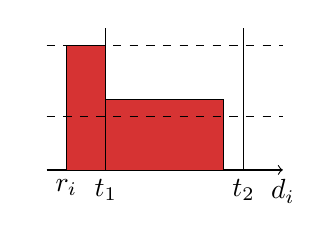
\begin{tikzpicture} [xscale=0.5,yscale=0.45]
      \node (O) at (0,0) {};
      \draw [->] (0,0) -- (6,0);
      \fill[red!80!black!80] (0.5,0) rectangle (1.5,3.5);
      \fill[red!80!black!80] (1.5,0) rectangle (4.5,2);
      \draw (0.5,0) node[below] {$r_i$};
      \draw (6,0) node[below] {$d_i$};
      \draw (1.5,0) node[below] {$t_1$} -- (1.5,4);
      \draw (5,0) node[below] {$t_2$} -- (5,4);
      \draw[dashed] (0,1.5) node[left] {$\bmin$} -- (6,1.5);
      \draw[dashed] (0,3.5) node[left] {$\bmax$} -- (6,3.5);
      \draw (0.5,0) -- (0.5,3.5) -- (1.5,3.5) -- (1.5,2) -- 
      (4.5,2) -- (4.5,0);
    \end{tikzpicture}
    &
      \onslide<2->{
      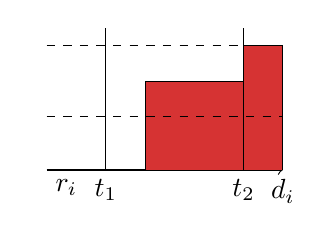
\begin{tikzpicture} [xscale=0.5,yscale=0.45]
        \node (O) at (0,0) {};
        \draw [->] (0,0) -- (6,0);
        \fill[red!80!black!80] (5,0) rectangle (6,3.5);
        \fill[red!80!black!80] (5,0) rectangle (2.5,2.5);
        \draw (0.5,0) node[below] {$r_i$};
        \draw (6,0) node[below] {$d_i$};
        \draw (1.5,0) node[below] {$t_1$} -- (1.5,4);
        \draw (5,0) node[below] {$t_2$} -- (5,4);
        \draw[dashed] (0,1.5) node[left] {$\bmin$} -- (6,1.5);
        \draw[dashed] (0,3.5) node[left] {$\bmax$} -- (6,3.5);
        \draw (6,0) -- (6,3.5) -- (5,3.5) -- (5,2.5) --
        (2.5,2.5) -- (2.5,0);
      \end{tikzpicture}

      ~~~~~~~~~~~~}
    \\
    \multicolumn{1}{c}{\small left-shifted} &
                                       \multicolumn{1}{c}{\only<2->{\small 
                                       right-shifted} }
  \end{tabular}
  
  \begin{overlayarea}{\textwidth}{3cm}
    \only<3-4>{
      \begin{tabular}{cc}
        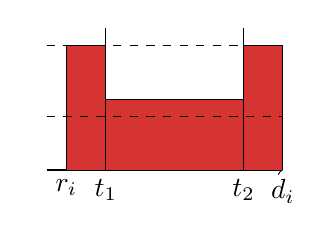
\begin{tikzpicture} [xscale=0.5,yscale=0.45]
          \node (O) at (0,0) {};
          \draw [->] (0,0) -- (6,0);
          \fill[red!80!black!80] (0.5,0) rectangle (1.5,3.5);
          \fill[red!80!black!80] (6,0) rectangle (5,3.5);
          \fill[red!80!black!80] (5,0) rectangle (1.5,2);
          \draw (0.5,0) node[below] {$r_i$};
          \draw (6,0) node[below] {$d_i$};
          \draw (1.5,0) node[below] {$t_1$} -- (1.5,4);
          \draw (5,0) node[below] {$t_2$} -- (5,4);
          \draw[dashed] (0,1.5) node[left] {$\bmin$} -- (6,1.5);
          \draw[dashed] (0,3.5) node[left] {$\bmax$} -- (6,3.5);
          \draw (0.5,0) -- (0.5,3.5) -- (1.5,3.5) -- (1.5,2) --
          (5,2) -- (5,3.5) -- (6,3.5) -- (6,0) ;
        \end{tikzpicture} 
        &
          \only<4>{
          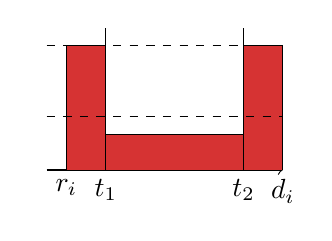
\begin{tikzpicture} [xscale=0.5,yscale=0.45]
                      \node (O) at (0,0) {};
          \draw [->] (0,0) -- (6,0);
          \fill[red!80!black!80] (0.5,0) rectangle (1.5,3.5);
          \fill[red!80!black!80] (6,0) rectangle (5,3.5);
          \fill[red!80!black!80] (5,0) rectangle (1.5,1);
          \draw (0.5,0) node[below] {$r_i$};
          \draw (6,0) node[below] {$d_i$};
          \draw (1.5,0) node[below] {$t_1$} -- (1.5,4);
          \draw (5,0) node[below] {$t_2$} -- (5,4);
          \draw[dashed] (0,1.5) node[left] {$\bmin$} -- (6,1.5);
          \draw[dashed] (0,3.5) node[left] {$\bmax$} -- (6,3.5);
          \draw (0.5,0) -- (0.5,3.5) -- (1.5,3.5) -- (1.5,1) --
          (5,1) -- (5,3.5) -- (6,3.5) -- (6,0) ;
          \end{tikzpicture}
          }
        \\
        \multicolumn{1}{c}{\small both-shifted 1} &
                                             \multicolumn{1}{c}{\only<4>{
                                             \small both-shifted 2}}
      \end{tabular}
    }
    \only<5-> {
      \begin{tabular}{cc}
        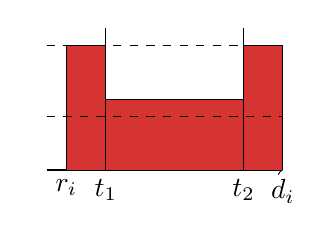
\begin{tikzpicture} [xscale=0.5,yscale=0.45]
          \node (O) at (0,0) {};
          \draw [->] (0,0) -- (6,0);
          \fill[red!80!black!80] (0.5,0) rectangle (1.5,3.5);
          \fill[red!80!black!80] (6,0) rectangle (5,3.5);
          \fill[red!80!black!80] (5,0) rectangle (1.5,2);
          \draw (0.5,0) node[below] {$r_i$};
          \draw (6,0) node[below] {$d_i$};
          \draw (1.5,0) node[below] {$t_1$} -- (1.5,4);
          \draw (5,0) node[below] {$t_2$} -- (5,4);
          \draw[dashed] (0,1.5) node[left] {$\bmin$} -- (6,1.5);
          \draw[dashed] (0,3.5) node[left] {$\bmax$} -- (6,3.5);
          \draw (0.5,0) -- (0.5,3.5) -- (1.5,3.5) -- (1.5,2) --
          (5,2) -- (5,3.5) -- (6,3.5) -- (6,0) ;
        \end{tikzpicture} 
        &
          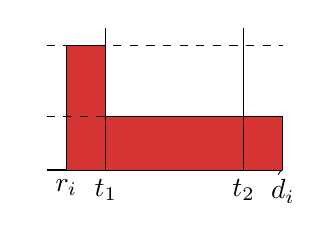
\begin{tikzpicture} [xscale=0.5,yscale=0.45]
            \node (O) at (0,0) {};
            \draw [->] (0,0) -- (6,0);
            \fill[red!80!black!80] (0.5,0) rectangle (1.5,3.5);
            \fill[red!80!black!80] (6,0) rectangle (1.5,1.5);
            \draw (0.5,0) node[below] {$r_i$};
            \draw (6,0) node[below] {$d_i$};
            \draw (1.5,0) node[below] {$t_1$} -- (1.5,4);
            \draw (5,0) node[below] {$t_2$} -- (5,4);
            \draw[dashed] (0,1.5) node[left] {$\bmin$} -- (6,1.5);
            \draw[dashed] (0,3.5) node[left] {$\bmax$} -- (6,3.5);
            \draw (0.5,0) -- (0.5,3.5) -- (1.5,3.5) -- (1.5,1.5) --
            (6,1.5)  -- (6,0) ;
          \end{tikzpicture}
        \\
        \multicolumn{1}{c}{\small both-shifted 1} &
                                             \multicolumn{1}{c}{
                                             \small both-shifted 2}
      \end{tabular}
    }
  \end{overlayarea}
\end{center}  
\end{frame}



\begin{frame}
  \frametitle{Energetic reasoning checker}
  We define the  slack function of interval $\inter$ as:
  \begin{gather}
    SL(t_1,t_2)={\color<2>{red}\text{ available space in
      }\inter}-{\color<2>{blue!50!}\text{ total mandatory }} \nonumber\\ 
        {\color<2>{blue!50!}\text{consumption in } \inter}\nonumber
  \end{gather}
  \begin{theorem}
    If there exists an interval on which the slack function is negative then there is no solution
  \end{theorem}
  \vfill
  \onslide<2>{
    \begin{center}
      \begin{tikzpicture}
        [transform shape,xscale=0.7,yscale=0.5]
        [inner sep=0pt]
        \node (O) at (0,0) {};
        \node[right of=O, node distance=6cm] (T) {};
        \node[right of=O, node distance=2cm] (t1) {};
        \node[right of=O, node distance=4cm] (t2) {};
        
        \draw[dashed] (0,4) node[left] {\Large$B$} -- (6,4);

        \draw[->] (O) -- (T);

        \draw[thick,red] (t1) -- (2,4.5);
        \draw[thick,red] (t2) -- (4,4.5);

        \draw[fill=blue!10!] (t1) node[above=2cm,left=0.6cm] {\color{blue!50!} \Large mandatory consumption} rectangle (4.5,4);
        \draw[pattern=north west lines, pattern color=red] (t1) rectangle (4,4) node[below=2cm,right=0.8cm] {\color{red} \Large available resource};
      \end{tikzpicture}
    \end{center}}
\end{frame}

\begin{frame}
  \frametitle{Relevant intervals}
  {\bf Question: } On which intervals $\inter$?\\
  \vfill
  $\rightarrow$ Analysis of the variation of the slack function\\
  \vfill
  \begin{block}{Slack function}
    \centering $SL(t_1,t_2)=B(t_2-t_1) - \sum_{i \in A} \bb$
  \end{block}
  \vspace{0.8cm}
  $\rightarrow$ Variation of $SL(t_1,t_2)$ depends on variation of 
  $\sum_{i \in A} \bb$
  \vfill 
\end{frame}


\subsubsection{Energetic reasoning filter}

\begin{frame}
  \frametitle{Time window adjustments}
  \vspace{0.4cm}
  \begin{center}
    \begin{tikzpicture}
  [yscale=0.5,xscale=0.9]
  \node[] (O) at (0,0) {};
  \node[label={[shift={(-0.4,-0.4)}]\small $b_i^{min}$}] (bmin) at (0,1) {};
  \node[label={[shift={(-0.4,-0.4)}]\small $b_i^{max}$}] (bmax) at (0,4) {};
  \node[label={[shift={(-0.4,-0.4)}]\small $B$}] (B) at (0,6) {};
  \node[label={[shift={(0,-0.8)}]\small $t_1$}] (t1) at (2.5,0) {}; 
  \node[label={[shift={(0,-0.8)}]\small $t_2$}] (t2) at (6,0) {};
  % \node[label={[shift={(0,-0.8)}]\small $d_i$}] (di) at (7,0) {};
  

  \onslide<5->{
    \draw[fill=gray!50!black!30] (4.25,1) --(6,1) -- (6,6) -- (2.5,6) --
    (2.5,1) --  (2.5,0)  -- (4.25,0) -- (4.25,1) -- cycle;
    \draw[pattern=north east lines, pattern color=blue!80!black!80] (4.25,0) rectangle (6,1);
    \draw[pattern=north east lines, pattern color=blue!80!black!80] (6,0) rectangle (7.5,4);
    \node[label={[shift={(0,-0.8)}]\small \color{red} $est_i$}] (ri) at
    (4.25,0) {}; 
    \draw(ri.south) -- (ri.center);
  } 
  \draw[->] (O.center) -- (8,0);
  \draw (O.south) -- (B.north);
  \draw (B.center) -- (8,6);
  \draw[dashed] (bmin.center) -- (8,1);
  \draw[dashed] (bmax.center) -- (8,4);
  
  % \draw(di.south) -- (di.center);
  \draw[thick] (t1.south) -- (2.5,6.1);
  \draw[thick] (t2.south) -- (6,6.1);
  
  % \onslide<1>{
  % \draw[fill=gray!50!black!30] (4.25,1) --(6,1) -- (6,6) -- (2.5,6) -- (2.5,1) --  cycle;
  % \draw[pattern=north west lines, pattern color=red!80!black!80] (6,0) rectangle (2.5,1);
  % \node[label={[shift={(0,-0.8)}]\small $est_i$}] (ri) at (1.5,0) {}; }

  \onslide<2>{
    \draw[fill=gray!50!black!30]  (6,6) rectangle (2.5,1)
    node[color=gray!50!black!80, midway,text width= 2cm]
    {\small $\sum_{i \neq j} \bb[j]$};
    \draw[pattern=north west lines, pattern
    color=red!80!black!80] (6,0) rectangle (2.5,1); 
    \node[label={[shift={(0,-0.8)}]\small $est_i$}] (ri) at (1.5,0) {}; 
    \draw(ri.south) -- (ri.center);}

\onslide<1-2>{
    \node[label={[shift={(0,-0.8)}]\small $est_i$}] (ri) at (1.5,0)
    {}; 
}

  \onslide<3-4>{
    \draw[fill=gray!50!black!30] (4.25,1) --(6,1) -- (6,6) -- (2.5,6) -- (2.5,1) --  cycle;
    \draw[pattern=north west lines, pattern
    color=red!80!black!80] (6,0) rectangle (2.5,1); 
    \node[label={[shift={(0,-0.8)}]\small $est_i$}] (ri) at (1.5,0){}; 
    \draw(ri.south) -- (ri.center);
    \draw[pattern=north east lines, pattern color=blue!80!black!80] (1.5,0) rectangle (2.5,4);}

  \onslide<3>{
    \draw[pattern=north east lines, pattern color=blue!80!black!80] (2.5,0) rectangle (6,3);
  }

  \onslide<4>{
    \draw[pattern=north east lines, pattern color=blue!80!black!80] (6,0) rectangle (7,4);
    \draw[pattern=north east lines, pattern color=blue!80!black!80] (2.5,0) rectangle (6,1.5);
  } 

\end{tikzpicture}

  \end{center}
  \vfill
  \begin{block}{Adjustments}
    if {\color<1-3>{red!80!black!80} available space for $i$}$<${\color<2-3>{blue!80!black} consumption of $i$ starting at $r_i$}  then
    \[\color<4>{blue!80!black}r_i \text{ can be adjusted}\]
  \end{block}
  \vfill
\end{frame}

\subsubsection{Other filtering algorithms}
\begin{frame}{Other filtering algorithms}

\end{frame}
\subsection{Mixed Integer Linear Program}

\begin{frame}{Justification of event-based model}

\end{frame}
\begin{frame}{Start/End model?}

\end{frame}


\begin{frame}
  \frametitle{An event-based formulation}
  {\small \it Adaptation of a model for the RCPSP {\color{gray!50!black!50} \it [Koné et al., 2011]}}
  \vfill
  \begin{block}{Variables}
    \begin{itemize}
    \item  $t_e$ represents the event (start or end time)
      \vspace{0.3cm}
    \item $z_{ie}=\left\{
        \begin{array}{ll}
          1 & \text{if $i$ is in process during $[t_{e},t_{e+1}]$}\\
          0 & \text{sinon}
        \end{array}
      \right.
      $
      \vspace{0.3cm}
    \item $B_{ie}$: resource quantity consumed by $i$ in $\inter[t_e][t_{e+1}]$
      \vspace{0.3cm}
    \item $W_{ie}$: energy brought to $i$ in $\inter[t_e][t_{e+1}]$   
    \end{itemize}
  \end{block}
\end{frame}
\subsection{Computational results}
\begin{frame}
  \frametitle{Computational results}
  \begin{block}{Instance generation}
    \begin{itemize}
    \item 5 instances 10, 60 tasks, 10 instances of 20, 25, 30 tasks. 
    \item random  $a_i$ and $c_i,\ \forall i \in A$, in ${[}1,10{]}$ and $W_i$ in ${[}0,f_i(W_i){]}$
    \end{itemize}
  \end{block}
  \begin{block}{Configuration}
    \begin{itemize}
    \item Intel Core i7-4770 processor with 4 cores and 8Go of RAM
    \item OS: 64-bit Ubuntu 12.04
    \item MILP resolution: CPLEX 12.6  
    \item BB : C++ and CPLEX at each leaf
    \item time limit: 7200 seconds
    \end{itemize}
  \end{block}
  

\end{frame}


\begin{frame}
  \frametitle{Computational results}
  \begin{figure}[!htb]
    \centering
    \includegraphics[width=0.9\linewidth]{figures/BB_time.png}
    \caption{Results of experiments for MILP model and hybrid branch-and-bound 
      for various parameters $\epsilon$ (CPU time in sec.)}
  \end{figure}

\end{frame}


\begin{frame}
  \frametitle{Computational results}
  \begin{figure}[!htb]
    \centering
    \includegraphics[width=0.9\linewidth]{figures/BB_solved.png}
    \caption{Percentage of solved instances for MILP model and hybrid 
      branch-and-bound (\% of solved instances)}
  \end{figure}
\vfill
\end{frame}